\section{Transformace souřadnic}

Definovat chování motoru lze zapsáním rovnic pro každou z fází (u 3 fázových motorů je tento prostor popisován jako $abc$ souřadnice), tento popis není pro řízení příliš praktický, i proto, že pokud není vyveden střední vodič z motoru je jeden ze stavů redundantní. Proto motor popisujeme buď v $\alpha \beta $ souřadnicích nebo $dq$. Rozdíl $dq$ oproti $\alpha \beta$ je že souřadnice rotují úhlovou rychlostí $\omega_{fr}$, tu zpravidla volíme jako stejnou jako úhlovou rychlost napájení $\omega_e$. Díky tomu jsou časové průběhy stavových proměnných (napětí, proud...) konstantní v ustáleném stavu. To je výhodné pro vybrané přístupy k řízení, dochází k zjednodušení návrhu regulátoru.

Pokud je vinutí motoru zapojeno do hvězdy s vyvedeným středem je úplné popsání motoru ještě souřadnice 0, tyto prostory se označují jako  $\alpha \beta 0$  nebo dq0 souřadnicové systémy. V těchto souřadnicích  0 souřadnice reprezentuje proud středním vodičem.

Pro 5-fázové je nutné transformace rozšířit o další 2 dimenze získáváme prostor s  4 souřadnicemi pokud není vyveden střední vodič a 5 pro plný popis.
% Konkrétní zvolené transformaci se věnuji v kapitole \ref{kap:transformace}.



U pětifázových motorů potřebujme pro návrh vektorového řízení reprezentaci v $dq$, tedy průmět do 2 rotujících kolmých souřadnic. V nejjednodušší verzi řízení postačují pouze 2. U vícefázových motorů pokud jsou řízeny pouze v $dq$, tak dojde ke generování 3. harmonické a jejich násobků, ta je pro pohon nežádoucí, způsobuje harmonické rušení a tím ztráty\cite{letadla},\cite{analyseOfMultiphase}. Proto se další dvojice souřadnic reprezentuje právě chování 3. harmonických. Tato rovina je označována jako $dq_3$.  



\subsection{Transformace \texorpdfstring{$dq_{1,3}$}{dq 1,3}}
\label{kap:transformace}
 

Transformace do $dq_{1,3}$, umožňuje v souřadnicích $dq_ 1$ kontrolovat první harmonickou a její $10n\pm1$ násobky a v souřadnicích $dq_3$  3. harmonickou s $10n\pm3$ násobky 1.harmonické. \cite{analyseOfMultiphase}




\begin{figure}[h]
     \centering
     % První obrázek
     \begin{subfigure}[b]{0.45\textwidth}
         \centering
         \input{obrazky/abframe1.tex}
         \caption{Prostor 1.harmonické }
         \label{fig:vlevo}
     \end{subfigure}
     \hfill % Vytvoří mezeru mezi obrázky
     % Druhý obrázek
     \begin{subfigure}[b]{0.45\textwidth}
         \centering
         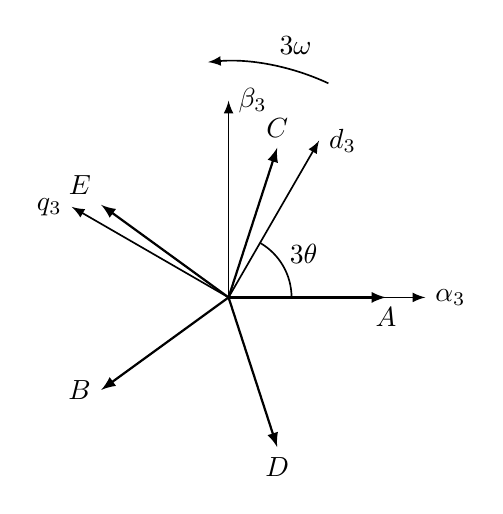
\begin{tikzpicture}[>=latex, line width=0.6pt]
\begin{scope}[shift={(7,0)}]
    % Osy alpha a beta
    \draw[->] (0,0) -- (2.5,0) node[right] {$\alpha_3$};
    \draw[->] (0,0) -- (0,2.5) node[right] {$\beta_3$};
    
    % Vektory fází A-E
    \draw[->, thick] (0,0) -- (0:2) node[below] {$A$};
    \draw[->, thick] (0,0) -- (216:2) node[left] {$B$};
    \draw[->, thick] (0,0) -- (72:2) node[above] {$C$};
    \draw[->, thick] (0,0) -- (288:2) node[below] {$D$};
    \draw[->, thick] (0,0) -- (144:2) node[above left] {$E$};
    
    % d-q soustava
    \def\threetheta{60}
    \draw[->] (0,0) -- (\threetheta:2.3) node[right] {$d_3$};
    \draw[->, shift={(0,0)}] (0,0) -- (\threetheta+90:2.3) node[left] {$q_3$};
    
    % Úhel 3*theta
    \draw (\threetheta:0.8) arc (\threetheta:0:0.8);
    \node at (30:1.1) {$3\theta$};
    
    % ŠIPKA 3*OMEGA - nyní na poloměru 3.0 (velmi daleko)
    \draw[->] (65:3.0) arc (65:95:3.0) node[midway, above right] {$3\omega$};
    
\end{scope}

\end{tikzpicture}
         \caption{Prostor 3.harmonické}
         \label{fig:vpravo}
     \end{subfigure}

     \caption{Ukázka souřadnic $\alpha \, \beta$ a $dq$}
     \label{fig:ukazka alfa beta 13}
\end{figure}




V \cite{analyseOfMultiphase} je pro převod z $abcde$ do $\alpha \beta_{1,3}$ použita rozšířená Clarkova transformace popsaná rovnicemi  \ref{eq:acbTOab1} až \ref{eq:acbTOab3}, kde $f_a-f_e$ odpovídají hodnotám v $abcde$ souřadnicích, reálná složka výsledku je potom $\alpha$ souřadnicí a imaginární $\beta$. Konstanta $\frac{2}{5}$ zajišťuje zachování velikosti amplitudy.

\begin{equation}
\label{eq:acbTOab1}
f_{\alpha_1 \beta_1 } \equiv \frac{2}{5} \left( f_{a} + a_5 f_{b} + a_5^2 f_{c} + a_5^3 f_{d} + a_5^4 f_{e} \right)
\end{equation}

\begin{equation}
    \label{eq:abc to 0}
    f_{\alpha_3 \beta_3 } \equiv \frac{2}{5} \left( f_{a} + a_5 f_{c} + a_5^2 f_{e} + a_5^3 f_{b} + a_5^4 f_{d} \right)
\end{equation}

\begin{equation}   
    \label{eq:acbTOab3}
    \begin{gathered}
        f_0=\frac{1}{5}\left( f_a +f_b+f_c+f_d+f_e\right)\\
a_5=e^{j2\pi/5}
\end{gathered}
\end{equation}


Z  $\alpha \beta _{1,3}$ je pak možné převést proměnné do rotujících souřadnic $dq_{1,3}$ použitím rovnic \ref{eq:ab1to dq1} a \ref{eq:ab3to dq3}, kde $\theta$ odpovídá úhlu mezi statickými a rotujícími $dq_1$ souřadnicemi, lze spočítat jako $\theta= \omega_{fr} \cdot t $, většinou je aproximován z měřených parametrů motoru. Souřadnice $dq_1$ rotují potom na stejné rychlosti jako 1. harmonická napětí a $dq_3$ třikrát rychleji.\cite{analyseOfMultiphase} \cite{letadla}

\begin{equation}
    \label{eq:ab1to dq1}
    f_{d_1 q_1}= f_{\alpha_1 \beta_1} \cdot e^{-j\theta}
\end{equation}


\begin{equation}
    \label{eq:ab3to dq3}
    f_{d_3 q_3}= f_{\alpha_3 \beta_3} \cdot e^{-j3\theta}
\end{equation}

\subsection{Převedení transformace do maticového tvaru}
Pro jednodušší práci jsem vztahy přepsal do maticových operací a vyhnul se použití komplexních čísel rozepsáním $d$ a $q$  jako další prvky, pro úplnost jsem také přidal 0 složku. Výpočet 0 složky vychází z rovnice \ref{eq:acbTOab3}, je kolmá na rovinu $\alpha \beta1$, tudíž se u ní neprojevuje rotace souřadnic. Nulová složka je nutná pro počítání inverzních matic pro zpětný převod. Matice $K_{s0}$ slouží pro převod z $abcde$ do $\alpha \beta _{1,3}0$. 



\begin{equation}
    \label{eq:Ks}
    \begin{bmatrix}
        f_{\alpha_1} \\ f_{\beta_1}\\ f_{\alpha_3} \\ f_{\beta_3}\\f_0
    \end{bmatrix}
    = 
    \underbrace{
        \frac{2}{5}
        \begin{bmatrix} 
            1 & \cos(\frac{2\pi}{5}) & \cos(\frac{4\pi}{5}) & \cos(\frac{6\pi}{5}) & \cos(\frac{8\pi}{5}) \\ 
            0 & \sin(\frac{2\pi}{5}) & \sin(\frac{4\pi}{5}) & \sin(\frac{6\pi}{5}) & \sin(\frac{8\pi}{5}) \\ 
            1 & \cos(\frac{6\pi}{5}) & \cos(\frac{2\pi}{5}) & \cos(\frac{8\pi}{5}) & \cos(\frac{4\pi}{5}) \\ 
            0 & \sin(\frac{6\pi}{5}) & \sin(\frac{2\pi}{5}) & \sin(\frac{8\pi}{5}) & \sin(\frac{4\pi}{5}) \\
            \frac{1}{2} & \frac{1}{2} &\frac{1}{2} &\frac{1}{2} &\frac{1}{2} 
        \end{bmatrix}
        }_{K_{s0}}
        \begin{bmatrix}
            f_a\\ f_b \\ f_c \\ f_d\\ f_e
        \end{bmatrix}
    \end{equation}
    
    Rotaci souřadnic jde vyjádřit maticí  $R_0(\theta)$, s její pomocí provádím transformaci z  $\alpha \beta_{1,3}0$ do $dq_{1,3}0$.
    \begin{equation}
        \label{eq:Rmatice}
    \begin{bmatrix}
        f_{d_1} \\ f_{q_1}\\ f_{d_3} \\ f_{q_3}\\f_0
    \end{bmatrix}
    = 
    \underbrace{
        \begin{bmatrix} 
            \cos(\theta) & \sin(\theta) & 0 & 0  & 0\\ 
            -\sin(\theta) & \cos(\theta) & 0 & 0 & 0\\ 
            0 & 0 & \cos(3\theta) & \sin(3\theta) & 0\\ 
            0 & 0 & -\sin(3\theta) & \cos(3\theta) & 0\\
            0 & 0 & 0  & 0  & 1
        \end{bmatrix}
        }_{R_0(\theta)}
        \begin{bmatrix}
            f_{\alpha_1} \\ f_{\beta_1}\\ f_{\alpha_3} \\ f_{\beta_3}\\f_0
        \end{bmatrix}
    \end{equation}
    
    Měřená data je často vhodné transformovat přímo do $dq_{1,3}0$, proto zavádím matici  $K_{r0}(\theta)$ která slouží  pro přímý převod z $abcde$ do rotujících souřadnic $dq_{1,3}0$.
\begin{equation}
    f_{dq_{1,3}}= \underbrace{R_0(\theta) \cdot K_{S0}}_{K_{R0}(\theta)} \cdot f_{abcde}
\end{equation}

\begin{equation}
\label{mat:Kr}
 K_{r0}=\frac{2}{5}\resizebox{0.8\textwidth}{!}{$
    \left( \begin{array}{ccccc}
    \cos \left(\theta \right) & \cos \left(\theta -\frac{2\,\pi }{5}\right) & -\cos \left(\theta +\frac{\pi }{5}\right) & -\cos \left(\theta -\frac{\pi }{5}\right) & \cos \left(\theta +\frac{2\,\pi }{5}\right)\\
    -\sin \left(\theta \right) & \cos \left(\theta +\frac{\pi }{10}\right) & \sin \left(\theta +\frac{\pi }{5}\right) & -\cos \left(\theta +\frac{3\,\pi }{10}\right) & -\sin \left(\theta +\frac{2\,\pi }{5}\right)\\
    \cos \left(3\,\theta \right) & -\cos \left(3\,\theta -\frac{\pi }{5}\right) & \cos \left(3\,\theta -\frac{2\,\pi }{5}\right) & \cos \left(3\,\theta +\frac{2\,\pi }{5}\right) & -\cos \left(3\,\theta +\frac{\pi }{5}\right)\\
    -\sin \left(3\,\theta \right) & -\cos \left(3\,\theta +\frac{3\,\pi }{10}\right) & \cos \left(3\,\theta +\frac{\pi }{10}\right) & -\sin \left(3\,\theta +\frac{2\,\pi }{5}\right) & \sin \left(3\,\theta +\frac{\pi }{5}\right)\\
    \frac{1}{2} & \frac{1}{2} & \frac{1}{2} & \frac{1}{2} & \frac{1}{2}
\end{array} \right)
$}
\end{equation}

Pro převod opačným směrem, tedy například z $dq_{1,3}0$ do $abcde$, stačí použít inverzi požadované matice. Tyto inverze jsem spočítal dopředu aby výpočet inverzí nezpomaloval chod řídícího programu. Aby bylo zřejmé že se jedná o již spočítané inverzní matice a ne matematickou operaci, budu tyto matice označovat jako $K_{s0}^{inv}$,$R_{0}^{inv}(\theta)$ a $K_{R}^{inv}(\theta)$. Například pro převod  $dq_{1,3}$ do $abcde$ lze použít vztah \ref{eq:tqrsfomace zpet}, kde  $K_{R0}^{inv}(\theta)=K_{R0}^{-1}(\theta)$.  

\begin{equation}
    \label{eq:tqrsfomace zpet}
    f_{abcde}=K_{R0}^{inv} \cdot f_{dq_{1,3}0}
\end{equation}


\begin{equation}
    K_{r0}^{inv}=\left(\begin{array}{ccccc}
\cos \left(\theta \right) & -\sin \left(\theta \right) & \cos \left(3\,\theta \right) & -\sin \left(3\,\theta \right) & 1\\
\cos \left(\theta -\frac{2\,\pi }{5}\right) & \cos \left(\theta +\frac{\pi }{10}\right) & -\cos \left(3\,\theta -\frac{\pi }{5}\right) & -\cos \left(3\,\theta +\frac{3\,\pi }{10}\right) & 1\\
-\cos \left(\theta +\frac{\pi }{5}\right) & \sin \left(\theta +\frac{\pi }{5}\right) & \cos \left(3\,\theta -\frac{2\,\pi }{5}\right) & \cos \left(3\,\theta +\frac{\pi }{10}\right) & 1\\
-\cos \left(\theta -\frac{\pi }{5}\right) & -\cos \left(\theta +\frac{3\,\pi }{10}\right) & \cos \left(3\,\theta +\frac{2\,\pi }{5}\right) & -\sin \left(3\,\theta +\frac{2\,\pi }{5}\right) & 1\\
\cos \left(\theta +\frac{2\,\pi }{5}\right) & -\sin \left(\theta +\frac{2\,\pi }{5}\right) & -\cos \left(3\,\theta +\frac{\pi }{5}\right) & \sin \left(3\,\theta +\frac{\pi }{5}\right) & 1
\end{array}\right)
\end{equation}

\begin{equation}
    R^{inv}=\left(\begin{array}{cccc}
\cos \left(\theta \right) & -\sin \left(\theta \right) & 0 & 0\\
\sin \left(\theta \right) & \cos \left(\theta \right) & 0 & 0\\
0 & 0 & \cos \left(3\,\theta \right) & -\sin \left(3\,\theta \right)\\
0 & 0 & \sin \left(3\,\theta \right) & \cos \left(3\,\theta \right)
\end{array}\right)
\end{equation}


V této práci uvažuji zapojení do hvězdy bez vyvedeného středu, souřadnicová složka 0 je tedy  vždy rovna 0. Je tedy zbytečné ji dále používat, proto budou dále vystupovat převážně matice $K_s; K_r;K_{s}^{inv};K_{r}^{inv}$. Ty jsou submaticemi popsaných $K_{s0}; K_{r0};K_{s0-inv};K_{r0-inv}$ s vynechanými řádky případně sloupci které se vztahují právě k 0 složce.


Odvození a plné vyčíslení všech matic a submatic včetně jejich výpočtu je v odvozeni.mlx souboru, který je součástí elektronické přílohy.

%bez editace
\section{Motor}
Práce se zabývá řízením 5 fázového synchronního motoru s permanentními magnety, konkrétně IPMSM(Interior Permanent Magnet Synchronous Machine) tedy motor s magenty umístěnými uvnitř motor. Konkrétní parametry jsou shrnuty v tabulce~\ref{tab:param_motoru}.  


Njednoduššší konfikurace perifáorvé PMSM motoru má rotor motrou je permanntní magent. Na staroru je umístěno rovnoměrně po po $72\deg$ rozmístěno 5  satorových vinutí. Jdenolivé fáze jsou označeny a,b,c,d,e. Konce vinutí jsou spojeny do hvězdy.
Fáze jsou napájeny sřidavýn sinusovým napětím. Npětí na jdnotlivých fázácj sjou navájem posunutá také o 72 deg.

OBRÁZEK PMSM 


\begin{table}[h]
    \centering
    \begin{tabular}{|l|l|r l|}
    \hline
    Název proměnné & Zkratka & Hodnota & ~          \\     \hline
    Typ vinutí & -- & Star-wound        & ~       \\    
    Počet pólových dvojic & $p$ & 8     &~        \\    
    Toková vazba permanentního magnetu & $\psi_{\mathrm{PM}}$ & 0.04366& Wb            \\    
    Vlastní indukčnost statoru na fázi & $L_s$ & 0.0002& H        \\    
    Fluktuace indukčnosti statoru & $L_m$ & -0.00002 & H        \\    
    Vzájemná indukčnost statoru & $M_s$ & 0.00002 &H      \\    
    Odpor statoru na fázi & $R_s$ & 0.010087 & $\Omega$               \\
    \hline
    \end{tabular}
    \caption{Parametry synchronního motoru s permanentními magnety}
    \label{tab:param_motoru}
\end{table}
\subsection{Výhody vícefázových motorů}
%Multi-phase drives offer some distinct advantages over their three-phase drive counterparts. The major advantages of using a multi-phase machine instead of a three-phase machine are described in [17–42]: higher torque density [22–26]; reduced torque pulsations [1, 27]; greater fault tolerance [27–38]; reduction in the required rating per inverter leg (and therefore simpler and more reliable power conditioning equipment) [39, 40]; and better noise characteristics, higher phase, number yield smoother torque due to the simultaneous increase of the frequency of the torque pulsation, and reduction of the torque ripple magnitude [41, 42]. Multi-phase drives are still unsuitable for general purpose drives application and thus their application areas are restricted to some critical domains such as ship propulsion, more-electric aircraft, hybrid electric vehicles, electric traction, and battery powered electric vehicles [43–48]. The reasons behind this are primarily two-fold. In high power applications (i.e. ship propulsion), the use of multi-phase drives enables reduction of the required power rating per inverter leg (phase). This is a major advantage over the converter end side, as lower switch ratings can handle reduced per-phase power. In high power applications, series and/or parallel combinations of power electronics switches are required to process large amounts of power. The series/parallel combination of switches poses the problem of static and dynamic voltage and current sharing. Thus reduced per-phase power is very attractive in this application. In safety-critical applications (i.e. more-electric aircraft), the use of multi-phase drives enables greater fault tolerance, which is of paramount importance. It has been shown that the loss of one or two phases has little impact on drive behavior. Finally, in electric vehicles and hybrid electric vehicle applications, use of multi-phase drives for propulsion enables reduction of the required semiconductor switch current rating; although these drives are not characterized by high power, low voltage availability in vehicles makes the current high.\cite{WileyHigPer}

Vícefázové pohony mají oproti klasickým trojfázovým řadu výhod. Oproti klasickým 3 fázovým motorům dosahují výší výkonové hustoty (poměr maximálního generovaného výkonu k hmotnosti motoru, genrovaný  moment  méně osciluje, generuji méně šumu. Zároveň jsou je možné je provozovat i při poruše na jedné z fází\cite{}. Vícefázové pohony se nepoužívají pro běžné instalace, jejich využiji je především pro kritické aplikace, jako je například pohony lodí, eklektické letouny, elektromobily a lokomotivy. 

Výkon přenášený do mootru je rozdělen do více fází, to předsatvuje výhodu u pohonů z vysokým výkonem. Rordelení proudu do  vice větví zpusobobuje snížení maximálního proudu tekoucí jedou větví (fází) střídače. To snižuje požadavky na jednotlivé polovodičové snímače, čímž se snižují cena celého pohonu.  

Dalším využití vícefázový pohonu je potom v kritických aplikacích (např.~letouny). Vícefázové pohony zvládají bez větších obtíží fungovat i při výpadku jedné či dvou fází. \cite{WileyHigPer}

\subsection{Matematický model motoru}
\label{kap:model abcd}

Vztah mezi napětím a proudem lze vyjádřit  z rovnice \ref{eq:model abc u}, jako sučet ubynapětí zpusobeným odporem vinutí a  $\frac{d\psi_i}{dt}$ odpovídjícímu  derivacím magnetického toku statoru $\psi_i$.

Magentickáý tok statorm  je podle rovnice \ref{eq:fluxabc} závislý na proudech statorem,  matici vzájemných indukčností $L_S(\theta)$ a příspěvku od rotorovém magnetickém toku $\psi_{im}$ vtaženého ke statoru.


\cite{malab_motor},\cite{Model_5phase}

\begin{equation}
    \label{eq:model abc u}
    \begin{bmatrix}
        v_a \\ v_b \\ v_c \\ v_d \\ v_e
    \end{bmatrix}
    =
    R_S \cdot
    \begin{bmatrix}
        i_a \\ i_b \\ i_c \\ i_d \\ i_e
    \end{bmatrix}
    +
    \begin{bmatrix}
        \frac{d\psi_a}{dt} \\
    \frac{d\psi_b}{dt} \\
    \frac{d\psi_c}{dt} \\
    \frac{d\psi_d}{dt} \\
    \frac{d\psi_e}{dt}
\end{bmatrix}
\end{equation}

\begin{equation}
    \label{eq:fluxabc}
    \begin{bmatrix}
        \psi_a \\ \psi_b \\ \psi_c \\ \psi_d \\ \psi_e
    \end{bmatrix}
    =
    L_s(\theta)
    \begin{bmatrix}
        i_a \\ i_b \\ i_c \\ i_d \\ i_e
    \end{bmatrix}
    +
    \begin{bmatrix}
        \psi_{am} \\ \psi_{bm} \\ \psi_{cm} \\ \psi_{dm} \\ \psi_{em}
    \end{bmatrix}
\end{equation}


Přepočt magentického toku pemanrtního magnetu z na jehon staotrové přispěvky je možné momocí rovnice \ref{eq:flux rotace abc}. Tok je závislý na magnetickém toku rotoru vyvoleném permanentními magenty $\psi_{PM}$ rotoru a jeho natočení vuči jednolivým vinutím  $ \theta_r$ (rovnice \ref{eq:flux rotace abc}).

\begin{equation}
    \label{eq:flux rotace abc} 
    \begin{bmatrix}
        \psi_{am} \\
        \psi_{bm} \\
        \psi_{cm} \\
\psi_{dm} \\
\psi_{em}
\end{bmatrix} = 
\underbrace{
\begin{bmatrix}
\cos \theta_r \\
\cos(\theta_r - 2\pi/5) \\
\cos(\theta_r - 4\pi/5) \\
\cos(\theta_r + 4\pi/5) \\
\cos(\theta_r + 2\pi/5)
\end{bmatrix}}_\gamma
\cdot \Psi_{PM}
\end{equation}

Matice $L_S(\theta)$ je pak dána rovnicí \ref{eq:model abc induknost},kde matice $I$ je jednotková matice distribuující rozptzlovou iudukčncost jedolivých vinutí vinutí $L_{ls}$. Matice $M_{a5}$ ppřpočírává vzájmené indukčnosti staotrových cívek mezi sebou. Polsední člen přidává vzajemnou indukčnot ovlivněnoenzávisou na poloze rotoru, matice  $M_{b5}$ složí k přepočtu Indukčnostní a je funkcí $\theta$.  

\begin{equation}
    \label{eq:model abc induknost}
    L_{s}(\theta) = L_{ls}I + L_{A5}M_{a5} + L_{B}M_{b5}(\theta)
\end{equation}


\begin{equation}
    M_{a5}=
    \begin{bmatrix}
    1 & \cos\left(\frac{2\,\pi}{5}\right) & \cos\left(\frac{4\,\pi}{5}\right) & \cos\left(\frac{4\,\pi}{5}\right) & \cos\left(\frac{2\,\pi}{5}\right)\\ \cos\left(\frac{2\,\pi}{5}\right) & 1 & \cos\left(\frac{2\,\pi}{5}\right) & \cos\left(\frac{4\,\pi}{5}\right) & \cos\left(\frac{4\,\pi}{5}\right)\\ \cos\left(\frac{4\,\pi}{5}\right) & \cos\left(\frac{2\,\pi}{5}\right) & 1 & \cos\left(\frac{2\,\pi}{5}\right) & \cos\left(\frac{4\,\pi}{5}\right)\\ \cos\left(\frac{4\,\pi}{5}\right) & \cos\left(\frac{4\,\pi}{5}\right) & \cos\left(\frac{2\,\pi}{5}\right) & 1 & \cos\left(\frac{2\,\pi}{5}\right)\\ \cos\left(\frac{2\,\pi}{5}\right) & \cos\left(\frac{4\,\pi}{5}\right) & \cos\left(\frac{4\,\pi}{5}\right) & \cos\left(\frac{2\,\pi}{5}\right) & 1
    \end{bmatrix}
\end{equation}

\begin{equation}
        M_{b5}=
        \begin{bmatrix}
         \cos\left(2\,\theta \right) & \cos\left(\frac{2\,\pi}{5}-2\,\theta \right) & \cos\left(\frac{4\,\pi}{5}-2\,\theta \right) & \cos\left(\frac{4\,\pi}{5}+2\,\theta \right) & \cos\left(\frac{2\,\pi}{5}+2\,\theta \right)\\ \cos\left(\frac{2\,\pi}{5}-2\,\theta \right) & \cos\left(\frac{4\,\pi}{5}-2\,\theta \right) & \cos\left(\frac{4\,\pi}{5}+2\,\theta \right) & \cos\left(\frac{2\,\pi}{5}+2\,\theta \right) & \cos\left(2\,\theta \right)\\ \cos\left(\frac{4\,\pi}{5}-2\,\theta \right) & \cos\left(\frac{4\,\pi}{5}+2\,\theta \right) & \cos\left(\frac{2\,\pi}{5}+2\,\theta \right) & \cos\left(2\,\theta \right) & \cos\left(\frac{2\,\pi}{5}-2\,\theta \right)\\ \cos\left(\frac{4\,\pi}{5}+2\,\theta \right) & \cos\left(\frac{2\,\pi}{5}+2\,\theta \right) & \cos\left(2\,\theta \right) & \cos\left(\frac{2\,\pi}{5}-2\,\theta \right) & \cos\left(\frac{4\,\pi}{5}-2\,\theta \right)\\ \cos\left(\frac{2\,\pi}{5}+2\,\theta \right) & \cos\left(2\,\theta \right) & \cos\left(\frac{2\,\pi}{5}-2\,\theta \right) & \cos\left(\frac{4\,\pi}{5}-2\,\theta \right) & \cos\left(\frac{4\,\pi}{5}+2\,\theta \right) 
        \end{bmatrix}
\end{equation}



\subsection{Mechanika motoru}
\label{kap:mechanika}
Mechanicko část motoru lze modelovat jako rotující setrvačník s momentem setrvačnosti J, který je tlumen třením. Moment generovaný třením je lineárně závislý na otáčkách motoru koeficientem b. Motor vyvíjí moment o velikosti $T_m$ a je zatížen momentem $T_L$. Rovnice pohybu motoru je dána rovnicí \ref{eq:mechanika motor}. Pro potřeby modelování ji lze převést do tvaru \ref{eq:mechanika motor2}.

\begin{equation}
    \label{eq:mechanika motor}
J\dot{\omega} = T_m - T_L - b\,\omega
\end{equation}

\begin{equation}
        \label{eq:mechanika motor2}
\dot{\omega} = \frac{1}{J} \,(T_m - T_L - b\,\omega)
\end{equation}


\begin{equation}
    \dot{\psi} = \omega
\end{equation}

%
%\begin{equation}
%    \begin{pmatrix} \dot{\psi} \\ \dot{\omega} \end{pmatrix}
%    =
%    \begin{pmatrix} 0 & 1 \\ 0 & -\dfrac{b}{J} \end{pmatrix}
%    \begin{pmatrix} \psi \\ \omega \end{pmatrix}
%    +
%    \begin{pmatrix} 0 \\ \dfrac{1}{J} \end{pmatrix}
%    (T_m - T_L)
%\end{equation}




\subsection{Převod modelu motoru do $dq_{1,3}$} a $\alpha \beta_{1,3}$
Model z kapitoly \ref{kap:model abcd} obsahuje množství nelineárních funkcí, v maticích $L_s$ a $\gamma$. Tyto matice jsou funkcí úhlu $\theta$,který je proměnný v čase. Tento tvar popisu motoru není vhodný pro návrh řízení vektorovéh řízení motoru, i implementaci prostorově vektorové pulzně šířkové modulace. 

Cílem této kyitoly je  aplikoavt představenou transformaci na model motoru, ten nejdříve převedu do $\alpha \beta_{1,2}$ a následně $dq_{1,3}$. Získat tak model motoru v $dq_{1,3}$.

V kapitole je uvedno pouze odvození a ukazány  výsledky, násboení jedntlivýhc matic jsem provdel v prostředí matlab využitím sybmolzc toolboxu. Masobení jedtlivých maitic je součascí skriptu COJAVIM.m, ktrý je součastí elektronické přílohy.

\subsubsection{abcde do $\alpha \beta_{1,3}$}
Pro převod modelu do $\alpha \beta$ vyšel z rovnic v abcde ve kterých jsem nahradil stavy reprezentované v abcde  prostoru použitím vztahu $f_{abcde}=K_{S}^{inv} \cdot f_{\alpha \beta}$. 
U rovnice  pro statorové napětí \ref{eq:model abc u} po dosazení a roznásobí celé rovnice maticí $K_S$ získám vztah \ref{eq:model U allfa beta} který je podobný původnímu. 

\begin{equation}
    \label{eq:model U allfa beta}
    v_{s \alpha\beta{1,3}}=R_S \cdot i_{s \alpha \beta_{1,3}} + \frac{d\psi_{s\alpha \beta_{1,3}}}{dt}
\end{equation}

Rovnice pro statorový indukční tok vychází z \ref{eq:fluxabc} ze které dosazením získám rovnici \ref{eq:flux mezikrok}. Porotže   $ L_s(\theta)$ nené konstanou  ale maticí výraz rovnice je o něoc složitějš než v předchozím případě. Po roznásobení rovnice  maticí $K_S$ zleva a dostávm  vztah \ref{eq:flux alfa beta}.



\begin{equation}
    \label{eq:flux mezikrok}
    K_{S-inv} \cdot \psi_{\alpha \beta_{1,3}}=
    L_s(\theta)K_{s-inv} \cdot i_{\alpha \beta}+ K_{S-inv} \cdot \psi_{m \alpha \beta}
\end{equation}

\begin{equation}
    \label{eq:flux alfa beta}
    \psi_{\alpha \beta_{1,3}}=
    \underbrace{K_sL_s(\theta)K_{s-inv}}_{L_{\alpha \beta}} \cdot i_{\alpha \beta}+ \psi_{m \alpha \beta}
\end{equation}


Výpočet magenrického tokuk vzvolaného statorem spočivá pouze v dosazení.
\begin{equation}
    \label{eq:model rotorflux alfa beta}
    \psi_{m \alpha \beta}=\underbrace{K_S\gamma}_{\gamma_{s}} \cdot \Psi_{PM}
\end{equation}

\subsubsection{Převod modelu do dq}


Pro rovnici statorového napětí jsem vyšel z rovnice \ref{eq:model U allfa beta} v  $\alpha \beta$, všechny signály jsem převedl do $dq_{1,3}$ využitím vztahu $ f_{\alpha \beta 1,3} = R(\theta)^{ivn}  \cdot f_{dq13} $. Dosazením jsem získal rovnici \ref{eq:prevod1} a následným vyjádřením derivace součinu jsem došel k rovnici \ref{eq:prevod2}.


\begin{equation}
    \label{eq:prevod1}
    R_{inv} \cdot v_{dq}= R_S \cdot R(\theta)^{inv} \cdot i_{dq} + \frac{d}{dt} (R(\theta)^{inv} \cdot \psi_{dq}) 
\end{equation}


\begin{equation}
\label{eq:prevod2}
    R_{inv} \cdot v_{dq}= R_S \cdot R(\theta)^{inv} \cdot i_{dq} + \frac{d}{dt} R(\theta)^{inv} \cdot \psi_{dq} +  R(\theta)^{inv} \cdot \frac{d \cdot\psi_{dq}}{dt} 
\end{equation}

Rovnici \ref{eq:prevod2} pak vynásobím maticí R zleva. Čímž u většiny členů rovnice  získám  součin $R(\theta)^{inv} \cdot R $, který odpovídá jednotkové matici, pouze u členu $\psi_{dq}$ vznikne matice která není jednotková, tu označím jako E (rovnice \ref{eq:prevod3}). 

\begin{equation}
    \label{eq:prevod3}
    v_{dq}= R_S \cdot i_{dq} + \underbrace { R(\theta) \cdot \frac{d\cdot R(\theta)^{inv}}{dt}}_E  \cdot \psi_{dq} +  \frac{d \cdot\psi_{dq}}{dt} 
\end{equation}

Po dosazení $\theta=\omega_{fr}\cdot t$, do matice R jsem získal tvar k derivaci. Spočítáním derivace součinu $R_{inv} \cdot \psi_s$ a dalších úpravách jsem pak došel k rovnici \ref{eq:model dq v}. 

\begin{equation}
    \label{eq:model dq v}
    v_{dq}=R_S\cdot i_{dq}+\omega_{fr} 
    \underbrace{
    \begin{bmatrix}
    0 &-1&0&0\\
    1&0&0&0\\
    0&0&0&-3\\
    0&0&3&0 
    \end{bmatrix}}_{E}\psi_{sdq}+\frac{d\psi_{sdq}}{dt}
\end{equation}

Pro rovnici magnetický tok od rotoru jsem vyšel z rovnice \ref{eq:flux rotace abc} popisující tok v abcde, pokud je vektor magnetického toku zarovnaný s d souřadnicí (uhel natočení elektrického pole $\theta_e=0$ právě tehdy když je na fázi a maximální napětí), výraz po dosazení a vyjádření značně zjednoduší (vztah\ref{eq:flux rotace dq}), všechny složky vektoru $\gamma$ kromě první jsou nulové. 


\begin{equation}
    \label{eq:flux rotace dq}
    \psi_{r_{dq}}=K_R\cdot \gamma \cdot\Psi_{PM}
 =\begin{bmatrix}
        1&0&0&0
    \end{bmatrix}^T \cdot
    \Psi_{PM}
\end{equation}



U statorové magnetického toku je situace podobná jakou převodu do $\alpha \beta$. V případě transformace do $dq$ po roznásobení rovnice \ref{eq:model abc induknost} se celý výpočet $L_s$ významně zjednoduší na výraz \ref{eq: modle indukcnost dq}.       


\begin{equation}
    \psi_{sdq}=
     \underbrace{K_RL_sK_{R}^{inv}}_{L_{s-dq}} 
    \cdot i_{dq}+ \psi_{r_{dq}}
\end{equation}

\begin{equation}
\label{eq: modle indukcnost dq}
    L_{s_{dq}}=
    \begin{bmatrix}    
    \frac{5\,L_{\textrm{a5}} }{2}+\frac{5\,L_{\textrm{b5}} }{2}+L_{\textrm{ls}}  & 0 & 0 & 0\\
    0 & \frac{5\,L_{\textrm{a5}} }{2}-\frac{5\,L_{\textrm{b5}} }{2}+L_{\textrm{ls}}  & 0 & 0\\
    0 & 0 & L_{\textrm{ls}}  & 0\\
    0 & 0 & 0 & L_{\textrm{ls}} 
    \end{bmatrix}=
    \begin{bmatrix}
        L_{d1} &0&0&0\\
        0 &L_{q1}&0&0\\
        0 &0&L_{d3}&0\\
        0 &0&0&L_{q3}\\
    \end{bmatrix}
\end{equation}

%%% po dosazeni

Po dosazeni a úpravě rovnic statorového, rotorového indukčního toku a statorové  indukčnosti v dq, \ref{eq:flux rotace dq} až \ref{eq: modle indukcnost dq}, jsem získal rovnice \ref{eq:model dq flux final}. Pro z dalších výpočtu sem statorový indukční tok dosadil do rovnice statorového napětí \ref{eq:model dq v} čímž jsem došel ke vztahu \ref{eq:model dq v final}, který motor plně popisuje. Tyto rovnice jsou nezávislé na úhlu $\theta$, tedy i časově invariantní a všechny matice kromě matice E jsou diagonální. Získané rovnice jsou lineární a vhodné pro návrh řízení.



\begin{equation}
    \label{eq:model dq flux final}
    \psi_{s_{dq}}=
    \underbrace{
     \begin{bmatrix}    
        L_{d1} &0&0&0\\
        0 &L_{q1}&0&0\\
        0 &0&L_{d3}&0\\
        0 &0&0&L_{q3}\\
    \end{bmatrix}}_{L_{s_{dq}}}
    \cdot i_{dq}+ 
    \underbrace{
    \begin{bmatrix}
        1 \\ 0 \\0 \\0 
    \end{bmatrix}}_{\gamma_{dq}} \cdot \Psi_{PM}
\end{equation}



\begin{equation}
    \label{eq:model dq v final}
    v_{dq_{13}} = R_s i_{dq_{13}}+ \omega_{fr}E \left( L_{s}i_{dq_{13}} + \gamma \Psi_{PM}\right) + \frac{di_{dq_{13}}}{dt} Ls
\end{equation}

\section{Modulace SVPWM}
\label{kap:svm}
Pro modulaci požadovaného napětí je pro diplomovou práci zadána prostorově vektorová pulzně šířková modulace, v literatuře je nejčastěji označována zkratkou SVPWM (space vector pulse width modulation), nebo zkráceně SVM (space vector modulation). Prostorově vektorová pulzně šířková modulace je variantou modulace, která generuje sekvenci výstupů pro všech 5 fází přímo vektoru požadovaného napětí zadaného v $\alpha \beta$ souřadnicích. V této kapitole se věnuji popisu specifické verze  SVPWM pro pětifázový motor popsaný v kapitole \ref{kap:transformace}.\cite{analyseOfMultiphase}


Výstup modulátoru je označen jako v, v tomto  případě je výstupem 5 prvkový sloupcový vektor $u=[u_1, u_2,u_3,u_4,u_5]^T$, kde každý prvek vektoru odpovídá stavu odpovídající větve konvertoru. Pro dvouúrovňový měnič, který je v práci použit,  mohou jednotlivé prvky nabývat pouze hodnot  1 nebo -1. Pokud je $u_i= -1$ je připojená spodní větev konvertoru, napětí na výstupu konvertoru je napětí rovno $-v_{dc}/2$. Naopak pokud $u_i= 1$, pak je připojena horní větev měniče a výstup odpovídá $v_{dc}/2$. Pro vybraný střídač existuje 32 možných kombinací sepnutí spínačů, tedy 31 možných vektorů $u$, reprezentujících stavy přepínačů na jednotlivých fázích. Pokud tyto vektory s použitím představené transformace promítneme do $\alpha \beta_{1,3}$ prostoru, dostaneme možné výstupní vektory zobrazené na obrázku \ref{fig:svm} z nichž se 2 překrývají, jedná se o nulové vektory~($u_0=[-1,-1,-1,-1,-1]$ a $ u_{31}=[1,1,1,1,1]$).\cite{petros}\cite{analyseOfMultiphase}\cite{letadla}

\begin{figure}[htbp]
     \centering
     % První obrázek
     \begin{subfigure}[b]{0.45\textwidth}
         \centering
         \resizebox{\textwidth}{!}{
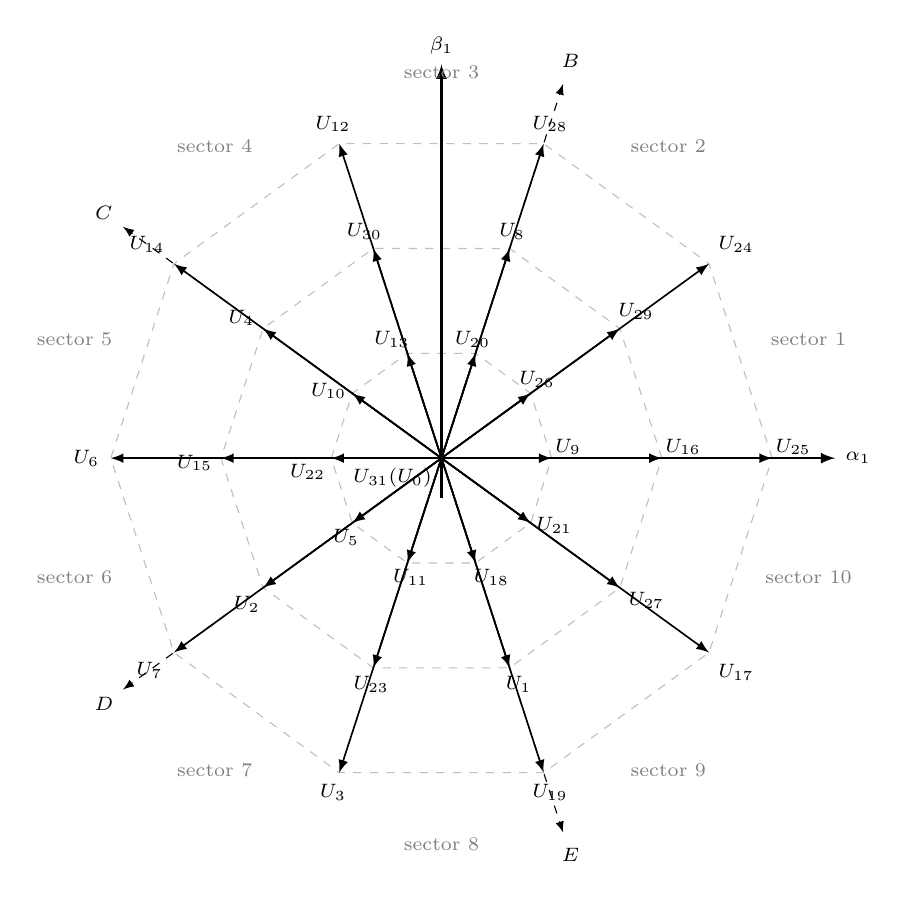
\begin{tikzpicture}[>=latex, font=\scriptsize]

    % Definice poloměrů
    \def\Rone{1.4}   
    \def\Rtwo{2.8}   
    \def\Rthree{4.2} 
    \def\Raxis{5.0}  

    % 1. Kreslení pozadí (čárkované desetiúhelníky)
    \foreach \r in {\Rone, \Rtwo, \Rthree} {
        \draw[dashed, gray!50] (0:\r) \foreach \x in {36,72,...,360} {-- (\x:\r)} -- cycle;
    }

    % 2. Hlavní osy
    \draw[->, thick] (-0.5,0) -- (\Raxis,0) node[right] {$\alpha_1$};
    \draw[->, thick] (0,-0.5) -- (0,\Raxis) node[above] {$\beta_1$};

    % Středový bod
    \node[below left] at (0,0) {$U_{31}(U_0)$};

    % 3. VEKTORY A POPISKY (Sjednocený styl pro osu alfa)

    % VNĚJŠÍ ÚROVEŇ (Level 3)
    \foreach \ang/\lab in {0/U_{25}, 36/U_{24}, 72/U_{28}, 108/U_{12}, 144/U_{14}, 180/U_6, 216/U_7, 252/U_3, 288/U_{19}, 324/U_{17}} {
        \draw[->, semithick] (0,0) -- (\ang:\Rthree);
        % Speciální podmínka pro úhel 0 (osa alfa), aby U25 bylo jako U9
        \ifnum\ang=0
            \node[anchor=south west, inner sep=1pt] at (\ang:\Rthree) {$\lab$};
        \else
            \node[anchor=\ang+180, inner sep=4pt] at (\ang:\Rthree) {$\lab$};
        \fi
    }

    % STŘEDNÍ ÚROVEŇ (Level 2)
    \foreach \ang/\lab in {0/U_{16}, 36/U_{29}, 72/U_8, 108/U_{30}, 144/U_4, 180/U_{15}, 216/U_2, 252/U_{23}, 288/U_1, 324/U_{27}} {
        \draw[->, semithick] (0,0) -- (\ang:\Rtwo);
        \ifnum\ang=0
            \node[anchor=south west, inner sep=1pt] at (\ang:\Rtwo) {$\lab$};
        \else
            \node[anchor=\ang+190, inner sep=3pt] at (\ang:\Rtwo) {$\lab$};
        \fi
    }

    % VNITŘNÍ ÚROVEŇ (Level 1)
    \foreach \ang/\lab in {0/U_9, 36/U_{26}, 72/U_{20}, 108/U_{13}, 144/U_{10}, 180/U_{22}, 216/U_5, 252/U_{11}, 288/U_{18}, 324/U_{21}} {
        \draw[->, semithick] (0,0) -- (\ang:\Rone);
        \ifnum\ang=0
            \node[anchor=south west, inner sep=1pt] at (\ang:\Rone) {$\lab$};
        \else
            \node[anchor=\ang+210, inner sep=2pt] at (\ang:\Rone) {$\lab$};
        \fi
    }

    % 4. Fázové osy a sektory
    \foreach \ang/\name in {72/B, 144/C, 216/D, 288/E} {
        \draw[->, dashed] (0,0) -- (\ang:\Raxis);
        \node at (\ang:\Raxis + 0.3) {$\name$};
    }
    
    \foreach \s/\ang in {1/18, 2/54, 3/90, 4/126, 5/162, 6/198, 7/234, 8/270, 9/306, 10/342} {
        \node[text=gray] at (\ang:\Rthree + 0.7) {sector \s};
    }


\end{tikzpicture}
}
         \caption{Prostor $\alpha \, \beta \,1$ }
         \label{fig:svm ab 1}
     \end{subfigure}
     \hfill % Vytvoří mezeru mezi obrázky
     % Druhý obrázek
     \begin{subfigure}[b]{0.45\textwidth}
         \centering
            \resizebox{\textwidth}{!}{
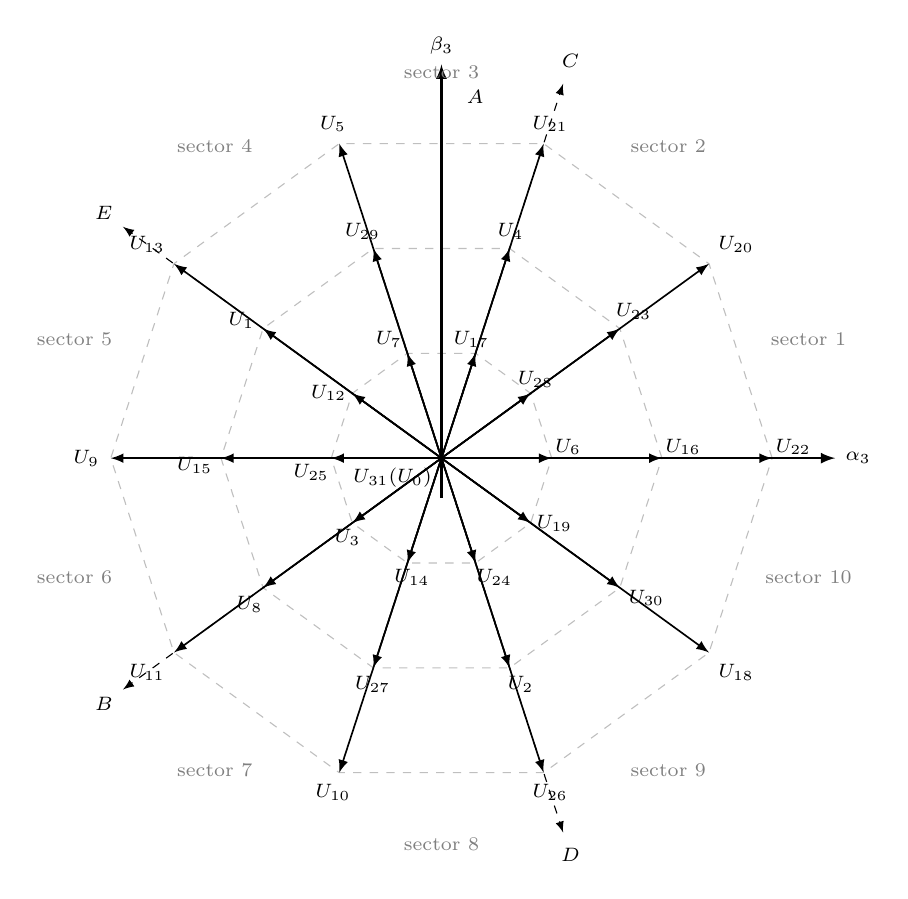
\begin{tikzpicture}[>=latex, font=\scriptsize]

    % Definice poloměrů
    \def\Rone{1.4}   
    \def\Rtwo{2.8}   
    \def\Rthree{4.2} 
    \def\Raxis{5.0}  

    % 1. Kreslení pozadí (čárkované desetiúhelníky)
    \foreach \r in {\Rone, \Rtwo, \Rthree} {
        \draw[dashed, gray!50] (0:\r) \foreach \x in {36,72,...,360} {-- (\x:\r)} -- cycle;
    }

    % 2. Hlavní osy (alfa 3 a beta 3)
    \draw[->, thick] (-0.5,0) -- (\Raxis,0) node[right] {$\alpha_3$};
    \draw[->, thick] (0,-0.5) -- (0,\Raxis) node[above] {$\beta_3$};

    % Středový bod
    \node[below left] at (0,0) {$U_{31}(U_0)$};

    % 3. VEKTORY A POPISKY PRO OBRÁZEK (b)

    % VNĚJŠÍ ÚROVEŇ (Level 3)
    \foreach \ang/\lab in {0/U_{22}, 36/U_{20}, 72/U_{21}, 108/U_{5}, 144/U_{13}, 180/U_9, 216/U_{11}, 252/U_{10}, 288/U_{26}, 324/U_{18}} {
        \draw[->, semithick] (0,0) -- (\ang:\Rthree);
        \ifnum\ang=0
            \node[anchor=south west, inner sep=1pt] at (\ang:\Rthree) {$\lab$};
        \else
            \node[anchor=\ang+180, inner sep=4pt] at (\ang:\Rthree) {$\lab$};
        \fi
    }

    % STŘEDNÍ ÚROVEŇ (Level 2)
    \foreach \ang/\lab in {0/U_{16}, 36/U_{23}, 72/U_4, 108/U_{29}, 144/U_{1}, 180/U_{15}, 216/U_{8}, 252/U_{27}, 288/U_{2}, 324/U_{30}} {
        \draw[->, semithick] (0,0) -- (\ang:\Rtwo);
        \ifnum\ang=0
            \node[anchor=south west, inner sep=1pt] at (\ang:\Rtwo) {$\lab$};
        \else
            \node[anchor=\ang+195, inner sep=3pt] at (\ang:\Rtwo) {$\lab$};
        \fi
    }

    % VNITŘNÍ ÚROVEŇ (Level 1)
    \foreach \ang/\lab in {0/U_6, 36/U_{28}, 72/U_{17}, 108/U_{7}, 144/U_{12}, 180/U_{25}, 216/U_3, 252/U_{14}, 288/U_{24}, 324/U_{19}} {
        \draw[->, semithick] (0,0) -- (\ang:\Rone);
        \ifnum\ang=0
            \node[anchor=south west, inner sep=1pt] at (\ang:\Rone) {$\lab$};
        \else
            \node[anchor=\ang+215, inner sep=2pt] at (\ang:\Rone) {$\lab$};
        \fi
    }

    % 4. Fázové osy pro (b) - A, C, E, B, D
    \node[anchor=north west] at (0.2, \Raxis-0.2) {$A$}; % Label u osy alfa
    \foreach \ang/\name in {72/C, 144/E, 216/B, 288/D} {
        \draw[->, dashed] (0,0) -- (\ang:\Raxis);
        \node at (\ang:\Raxis + 0.3) {$\name$};
    }
    
    % 5. Sektory
    \foreach \s/\ang in {1/18, 2/54, 3/90, 4/126, 5/162, 6/198, 7/234, 8/270, 9/306, 10/342} {
        \node[text=gray] at (\ang:\Rthree + 0.7) {sector \s};
    }



\end{tikzpicture}
}
         \caption{Prostor $\alpha \, \beta \,3$}
         \label{fig:svm ab 3}
     \end{subfigure}
     
     
    \caption{Rozložení výstupních vektorů }
    \label{fig:svm}
\end{figure}

Generované nenulové vektory dělíme do 3 kategorií, vektory s malou střední a velkou velikostí podle jejich velikosti $\alpha \beta_1$. Jak je vidět na obrázku \ref{fig:svm} vektory s malou délkou v $\alpha \beta_1$ odpovídají nejdelším v $\alpha\beta_3$.\cite{analyseOfMultiphase}

SVPWM se pomocí přepínáním těchto vektorů snaží během modulační periody generovat požadované napětí. Cílem je vybrat z generovaných vektorů 4 nenulové a určit jak dlouho mají být tyto vektory aplikované, tak abychom jejich součet přes jednu periodu modulace odpovídal žádanému vektoru napětí $U_{\alpha \beta_{1,3}}^*$. Pro dosažení reference v $\alpha \beta_1$ prostoru by stačily pouze 2 vektory. Protože je naším cílem sledovat referenci i 3. harmonické, náš referenční vektor je 4 prvkový a k jeho sledování jsou nutné 4 stupně volnosti(aplikační časy), jsme nuceni vybrat 4 vektory.\cite{petros}\cite{analyseOfMultiphase}\cite{letadla}

Pokud není vektor požadovaného napětí příliš dlouhý, je možné jej generovat libovolnou kombinací 4 nenulových vektorů. Existuje více možností jak volit vektory, které se pro generování použijí, například do pětiúhelníku. Já jsem se rozhodl pro volbu vektorů ohraničujících daný sektor a z nich ty se střední délkou, tím zajistím pouze 4 přepnutí při přechodu mezi vektory a také maximální modulační index pro napětí 1. harmonické.\cite{pentagram} \cite{multiphasePMSM} 


Jelikož je požadované napětí v $\alpha \beta_3$ ve většině případů menší než v  $\alpha \beta_1$ , tak vektory s malou délkou (nejdelší v $\alpha \beta_3$) nejsou využity. 


\subsection{Postup výpočtu}
Podle sektoru ve kterém se nachází reference v  $\alpha \beta_1$  jsou zvoleny vektory ohraničující tento prostor. Těch je celkem 6 z nich jsou vybrány ty s velkou a střední velikostí. Díky tomu je modulátor schopný dosáhnout nejvyššího možného generovaného napětí první harmonické (maximálního modulačního indexu).

\begin{figure}[htbp]
     \centering
     % První obrázek
     \begin{subfigure}[b]{0.45\textwidth}
         \centering
         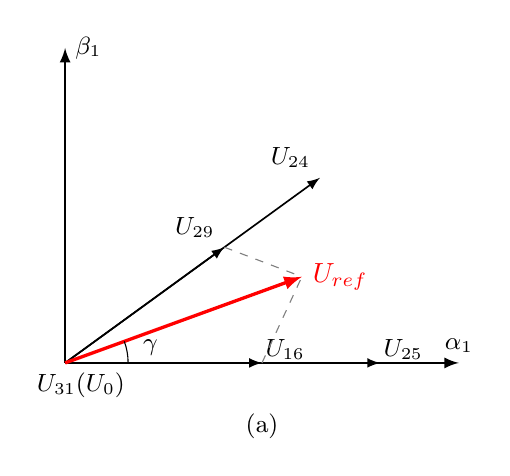
\begin{tikzpicture}[>=latex, font=\small]

    % Osy
    \draw[->, thick] (0,0) -- (5,0) node[above] {$\alpha_1$};
    \draw[->, thick] (0,0) -- (0,4) node[right] {$\beta_1$};
    \node[below] at (0.2,0) {$U_{31}(U_0)$};

    % Definice délek
    \def\Lone{2.5} 
    \def\Ltwo{4.0} 
    \def\Lref{3.2} 
    \def\angRef{20}

    % Vektory na ose alfa (U16, U25) - umístění nad šipkou
    \draw[->, semithick] (0,0) -- (\Lone,0) node[anchor=south west, inner sep=1pt] {$U_{16}$};
    \draw[->, semithick] (0,0) -- (\Ltwo,0) node[anchor=south west, inner sep=1pt] {$U_{25}$};

    % Vektory pod úhlem (U29, U24)
    \draw[->, semithick] (0,0) -- (36:\Lone) node[anchor=south east] {$U_{29}$};
    \draw[->, semithick] (0,0) -- (36:\Ltwo) node[anchor=south east] {$U_{24}$};

    % ČERVENÝ REFERENČNÍ VEKTOR Uref
    \draw[->, very thick, red] (0,0) -- (\angRef:\Lref) node[right, font=\bfseries] {$U_{ref}$};

    % Úhel gama
    \draw (0.8,0) arc (0:\angRef:0.8);
    \node at (10:1.1) {$\gamma$};

    % Konstrukční čáry
    \draw[dashed, gray] (36:\Lone) -- (\angRef:\Lref);
    \draw[dashed, gray] (\Lone,0) -- (\angRef:\Lref);

    \node at (2.5, -0.8) {(a)};

\end{tikzpicture}
         \caption{Prostor $\alpha \, \beta \,1$ }
         \label{fig:svm detail vlevo}
     \end{subfigure}
     \hfill % Vytvoří mezeru mezi obrázky
     % Druhý obrázek
     \begin{subfigure}[b]{0.45\textwidth}
         \centering
         \begin{tikzpicture}[>=latex, font=\small]

    % Osy
    \draw[->, thick] (-2.5,0) -- (4.5,0) node[below] {$\alpha_3$};
    \draw[->, thick] (0,-2.5) -- (0,4) node[right] {$\beta_3$};
    \node[anchor=south west, xshift=2pt] at (0,0) {$U_{31}(U_0)$};

    % Vektory na ose (U16 vpravo, U25 vlevo)
    \draw[->, semithick] (0,0) -- (2.8,0) node[anchor=south west, inner sep=1pt] {$U_{16}$};
    \draw[->, semithick] (0,0) -- (-1.8,0) node[anchor=north east] {$U_{25}$};

    % Šikmé vektory (U29 a U24)
    \draw[->, semithick] (0,0) -- (108:3.0) node[anchor=south east] {$U_{29}$};
    \draw[->, semithick] (0,0) -- (288:2.2) node[anchor=north west] {$U_{24}$};

    % ČERVENÝ REFERENČNÍ VEKTOR Uref3
    \def\angRefThree{130}
    \def\LrefThree{1.5}
    \draw[->, very thick, red] (0,0) -- (\angRefThree:\LrefThree) node[anchor=south east, font=\bfseries] {$U_{ref3}$};



\end{tikzpicture}
         \caption{Prostor $\alpha \, \beta \,3$}
         \label{fig:svm detail vpravo}
     \end{subfigure}
     
     \caption{Ukázka vybraných vektorů pro požadované napětí v prvním sektoru}
     \label{fig:svm_detail}
\end{figure}



Například pro požadované napětí v sektoru 1, vybereme výstupní vektory $U_{29}$, $U_{24}$, $U_{16}$, $U_{25}$ a nulové vektory $U_{0},U_{31}$. Detail vybraných vektorů je na obrázku \ref{fig:svm_detail}.

Pro tyto vybrané vektory je nutné spočítat časy $t_1 -t_4$, odpovídající době po kterou jsou dané vektory aplikované na výstup, tak aby jejich součet po dobu jedné periody odpovídal referenci.
Problém v $\alpha \beta_{1,3}$ lze zapsat rovnicí \ref{eq:svm cas ab}, kde $v_i - v_l$ jsou vybrané vektory napětí generované odpovídajícími vektory u  a $T_M$  vzorkovací perioda modulátoru.


\begin{equation}
    \label{eq:svm cas ab}
    \begin{gathered}
    V_{\alpha\beta_{13}}^* = \frac{t_1 \cdot v_i +t_2\cdot v_j + t_3\cdot v_k + t_4\cdot v_l}{T_M} \\ \\
    t_1+t_2+t_3+t_4 \leq T_M
    \end{gathered}
\end{equation}

Ve zmíněném případě, kdy je požadované napětí v prvním sektoru(obrázek \ref{fig:svm_detail}), jsou odpovídající vektory zapsané \ref{eq: prirazeni svm}.
\begin{equation}
\label{eq: prirazeni svm}
   \begin{gathered}
    v_i=v_{16};   
    v_j=v_{24};\\
    v_k=v_{25};
    v_l=v_{29}
   \end{gathered} 
\end{equation}

Maticově lze problém zapsat jako \ref{eq:maticove svm}, kde matici a jednotlivé sloupce reprezentují odpovídající napěťové  vektory. Matici A pak jde obecně vyjádřit jako \ref{eq:svm matica A}, kde n odpovídá číslu sektoru, $v_\alpha$ délce  napěťového vektoru se střední velikostí, $v_\beta$ s velkou a $V_\gamma$  s malou  velikostí . Je důležité dodržet pořadí vektorů stejné jako u příkladu zmíněného výše.\cite{analyseOfMultiphase}


\begin{equation}
    \label{eq:maticove svm}
    U_{\alpha \beta_{13}}^*=A \cdot 
    \begin{bmatrix}
        t_1\\t_2\\t_3\\t_4   
    \end{bmatrix}
\end{equation}
\begin{equation}    
    \label{eq:svm matica A}
    A_n = \frac{1}{T_M} \begin{bmatrix} 
    V_{\alpha} \cos \frac{(n-1)\pi}{5} & V_{\beta} \cos \frac{n\pi}{5} & V_{\beta} \cos \frac{(n-1)\pi}{5} & V_{\alpha} \cos \frac{n\pi}{5} \\ % asi lepsi cos(\gama + \frac{\pi}{5})
    V_{\alpha} \sin \frac{(n-1)\pi}{5} & V_{\beta} \sin \frac{n\pi}{5} & V_{\beta} \sin \frac{(n-1)\pi}{5} & V_{\alpha} \sin \frac{n\pi}{5} \\
    V_{\alpha} \cos \frac{3(n-1)\pi}{5} & -V_{\gamma} \cos \frac{3n\pi}{5} & -V_{\gamma} \cos \frac{3(n-1)\pi}{5} & V_{\alpha} \cos \frac{3n\pi}{5} \\
    V_{\alpha} \sin \frac{3(n-1)\pi}{5} & -V_{\gamma} \sin \frac{3n\pi}{5} & -V_{\gamma} \sin \frac{3(n-1)\pi}{5} & V_{\alpha} \sin \frac{3n\pi}{5}
    \end{bmatrix}
\end{equation}

Za předpokladu, že je známa matice $A$ a že existuje její inverze, je možné
rovnici \ref{eq:maticove svm} převést na explicitní řešení. Ze získaného vztahu
\ref{eq:svm casy final} lze již přímo spočítat hledané časy $t_1$ až $t_4$.

\begin{equation}
    \label{eq:svm casy final}
      \begin{bmatrix}
        t_1\\t_2\\t_3\\t_4   
    \end{bmatrix}
    = A_n^{-1}\cdot  U_{\alpha \beta_{1\,3}}^*
\end{equation}

Se znalostí potřebných vektorů a odpovídajících časů modulátor funguje podobně jako u 3fázové varianty SVPWM, vektory jsou aplikovány v pořadí aby se minimalizoval počet spínání tranzistorů, zbytek periody jsou potom aplikovány nulové vektory. Pro moji aplikaci použiji symetrickou sekvenci s použitím obou nulových vektorů. Podrobněji je aplikování vektorů popsáno v kapitole \ref{kap:vyvedeni}.